%================================================================
%\chapter{Analysis of the Hodgkin-Huxley Model}
\chapter{Analysis of the Neuroscientific Models}
%================================================================

%================================================================
\section{The Hodgkin-Huxley Model}
%================================================================

create the observed data

summary statistics of observation 

summary statistics from prior predictive

weights

(observed data with noise; same as above)

%================================================================
\section{The Brunel Network Model}
%================================================================

create the observed data

summary statistics of observation 

summary statistics from prior predictive

weights


%================================================================
\chapter{Parameter Identification with REJ-ABC}
%================================================================

%================================================================
\section{ABC Settings for Identification of Hodgkin-Huxley Parameters}
%================================================================


\begin{figure}[H]
    \centering
    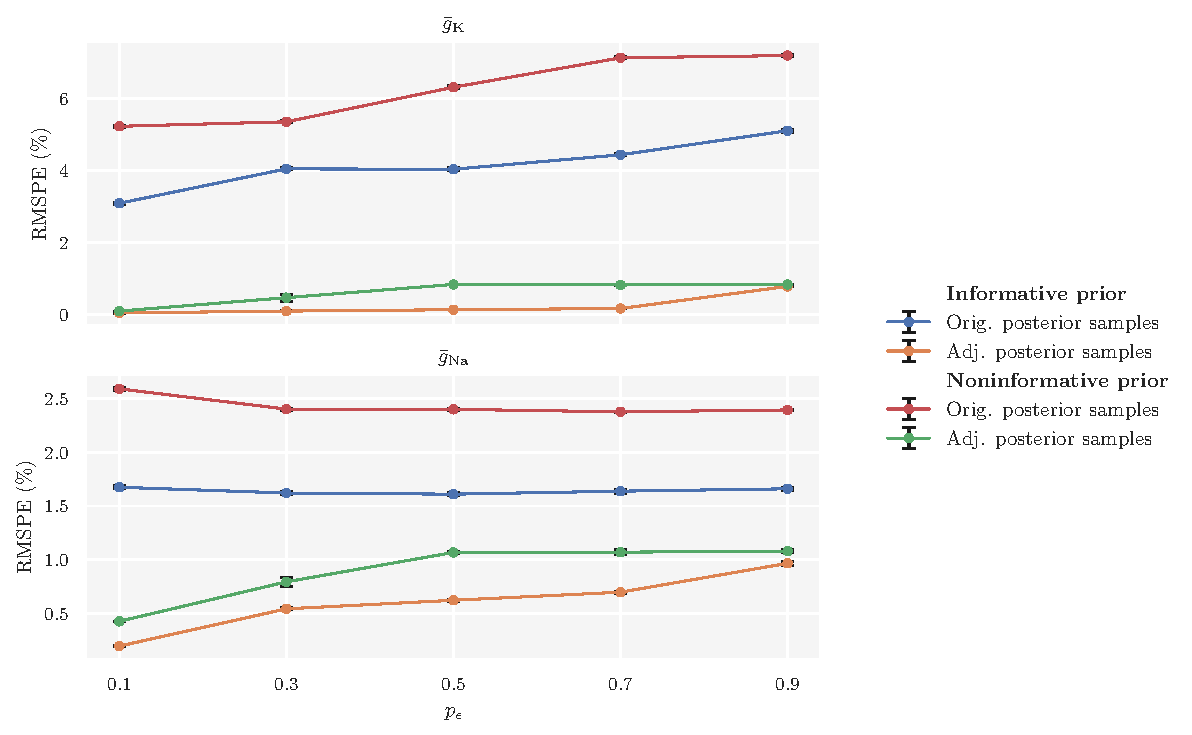
\includegraphics[scale=1]{RMSPE_vs_quantile}
    \caption{caption}
    \label{fig:fig1}
\end{figure} 


show how Hodgkin–Huxley model is more tightly constrained by increasing numbers of data features

We also inferred HH parameters for 8 in vitro recordings from the Allen Cell Types database using the same current-clamp stimulation protocol as in our model [60, 70] (Fig. 4F, Supplementary Fig. 8). In each case, simulations based on the SNPE-inferred posterior closely resembled the original data (Fig. 4F). We note that while inferred parameters differed across recordings, some parameters (the spike threshold, the density of sodium channels, the membrane reversal potential and the density of potassium channels) were consistently more strongly constrained than others (the intrinsic neural noise, the adaptation time constant, the density of slow voltage-dependent channels and the leak conductance) (Supplementary Fig. 8). Overall, these results suggest that the electrophysiological responses measured by this current-clamp protocol can be approximated by a single-compartment HH model, and that SNPE can identify the admissible parameters.

%================================================================
\section{Rejection ABC Posteriors on Conductance Parameters}
%================================================================

%================================================================
\section{ABC Settings for Identification of Brunel Network Parameters}
%================================================================

%================================================================
\section{Rejection ABC Posteriors on Synaptic Weight Parameters}
%================================================================

%================================================================
\chapter{Markov Chain Monte Carlo ABC on the Models}
%================================================================